\section{Ambiente de Desenvolvimento}

\begin{frame}[fragile]{Dyalog APL}

    \begin{itemize}
        \item A empresa Dyalog disponibiliza um ambiente de desenvolvimento baseado em APL, livre para uso não comercial
        \pause

        \item A versão mais recente é a 19.0
        \pause

        \item Há implementações disponíveis para Windows, MacOS, Linux e Raspberry Pi
        \pause
 
        \item O download pode ser feito na página oficial: \href{dyalog.com}{dyalog.com}
        \pause

        \item Em ambiente Linux, uma vez instalado, pode-se iniciar uma nova sessão por meio do
            comando

            \inputsyntax{bash}{codes/dyalog.sh}
        \pause

        \item \textbf{Cuidado!} Não execute este comando agora (caso contrário você terá que
            matar o processo para encerrar a sessão!)

    \end{itemize}

\end{frame}

\begin{frame}[fragile]{Teclado APL}

    Para inserir os glifos APL é preciso ou um teclado especializado ou a instalação de um \textit{layout} compatível.
        \pause

    \begin{figure}
        \centering
        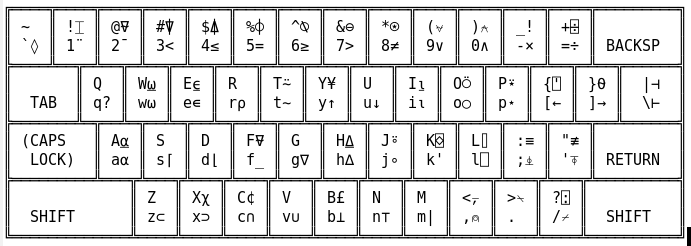
\includegraphics[scale=0.5]{figs/keyboard.png}

        \caption{\textit{Layout} de teclado GNU APL. Fonte: \href{https://lists.gnu.org/archive/html/bug-apl/2014-06/msg00261.html}{Bug-apl}}
    \end{figure}

\end{frame}

\begin{frame}[fragile]{Configuração de Layout no Ubuntu 20.04}

    \begin{enumerate}
        \item Nas configurações do sistema (\textit{Settings}), escolha a opção de região e
            linguagem (\textit{Region \& Language})
        \pause

        \item Adicione um segundo \textit{layout} qualquer (por exemplo, o \textit{layout} Braile)
            usando o símbolo \texttt{+} na lista de entradas (\textit{Input Sources})
        \pause

        \item Rode, no seu terminal, o comando

            \inputsyntax{bash}{codes/setlayout.sh}
        \pause

        \item Para tornar esta configuração permanente, adicione esta linha no arquivo
            \texttt{.bashrc}
        \pause

        \item Além do \textit{layout}, é recomendada a instalação da fonte \texttt{APL 385} para
            melhor visualização dos glifos
    \end{enumerate}
\end{frame}

\begin{frame}[fragile]{Inserção de glifos APL}

    \begin{itemize}
        \item Uma vez disponível o \textit{layout} APL, os glifos podem ser inseridos por meio
            de um combinação de teclas
        \pause

        \item A tecla \texttt{APL} deve ser combinada com uma outra tecla, ou com a tecla
            \texttt{Shift} e outra tecla
        \pause

        \item No \textit{layout} proposto, a tecla \texttt{APL} corresponde a tecla
            \texttt{Alt Gr}
        \pause

        \item Por exemplo, os glifos \texttt{⍴} e \texttt{⍒} podem ser inserido por meio das combinações
            \texttt{APL+p} e \texttt{APL+Shift+3}, respectivamente

        \pause

        \item Uma maneira alternativa é inserir os códigos unicode de cada caractere diretamente
            em seu editor

        \pause

        \item Este método dispensa a configuração do \textit{layout}, porém demanda a memorização
            dos códigos e do uso de mais teclas por caractere
    \end{itemize}

\end{frame}

\begin{frame}[fragile]{Encerrando a sessão do Dyalog}

    \begin{itemize}
        \item Uma vez instalado o \textit{layout}, é possível encerrar corretamente uma seção do Dyalog
        \pause

        \item Basta utilizar a função de sistema \texttt{OFF}
        \pause

        \item Em APL, as funções de sistema tem seus nomes prefixados pelo símbolo \texttt{⎕} (quad)
        \pause

        \item A dificuldade em encerrar a sessão citada anteriormente provém do fato da necessidade
            da inserção de um glifo para acessar a função de sistema, tarefa complicada sem o
            \textit{layout} previamente configurado

        \pause

        \item Portanto, basta invocar a função de sistema \texttt{OFF} em uma sessão ativa do Dyalog:

            \inputsyntax{apl}{codes/off.apl}

    \end{itemize}

\end{frame}

\begin{frame}[fragile]{Novo símbolo}

    \newAPLsymbol{⎕}{quad}{monádico}{Prefixo das funções de sistema}{U+2395}{[ ] <tab>}{APL + l}

\end{frame}

\begin{frame}[fragile]{TryAPL}

    \begin{itemize}
        \item A Dialog disponibiliza um ambiente online chamado TryAPL para que deseja conhecer a linguagem
        \pause

        \item Ela disponbiliza um modo de inserção baseado em uma combinação intuitiva de dois caracteres ASCII, seguidos de um TAB

        \begin{figure}
            \centering
            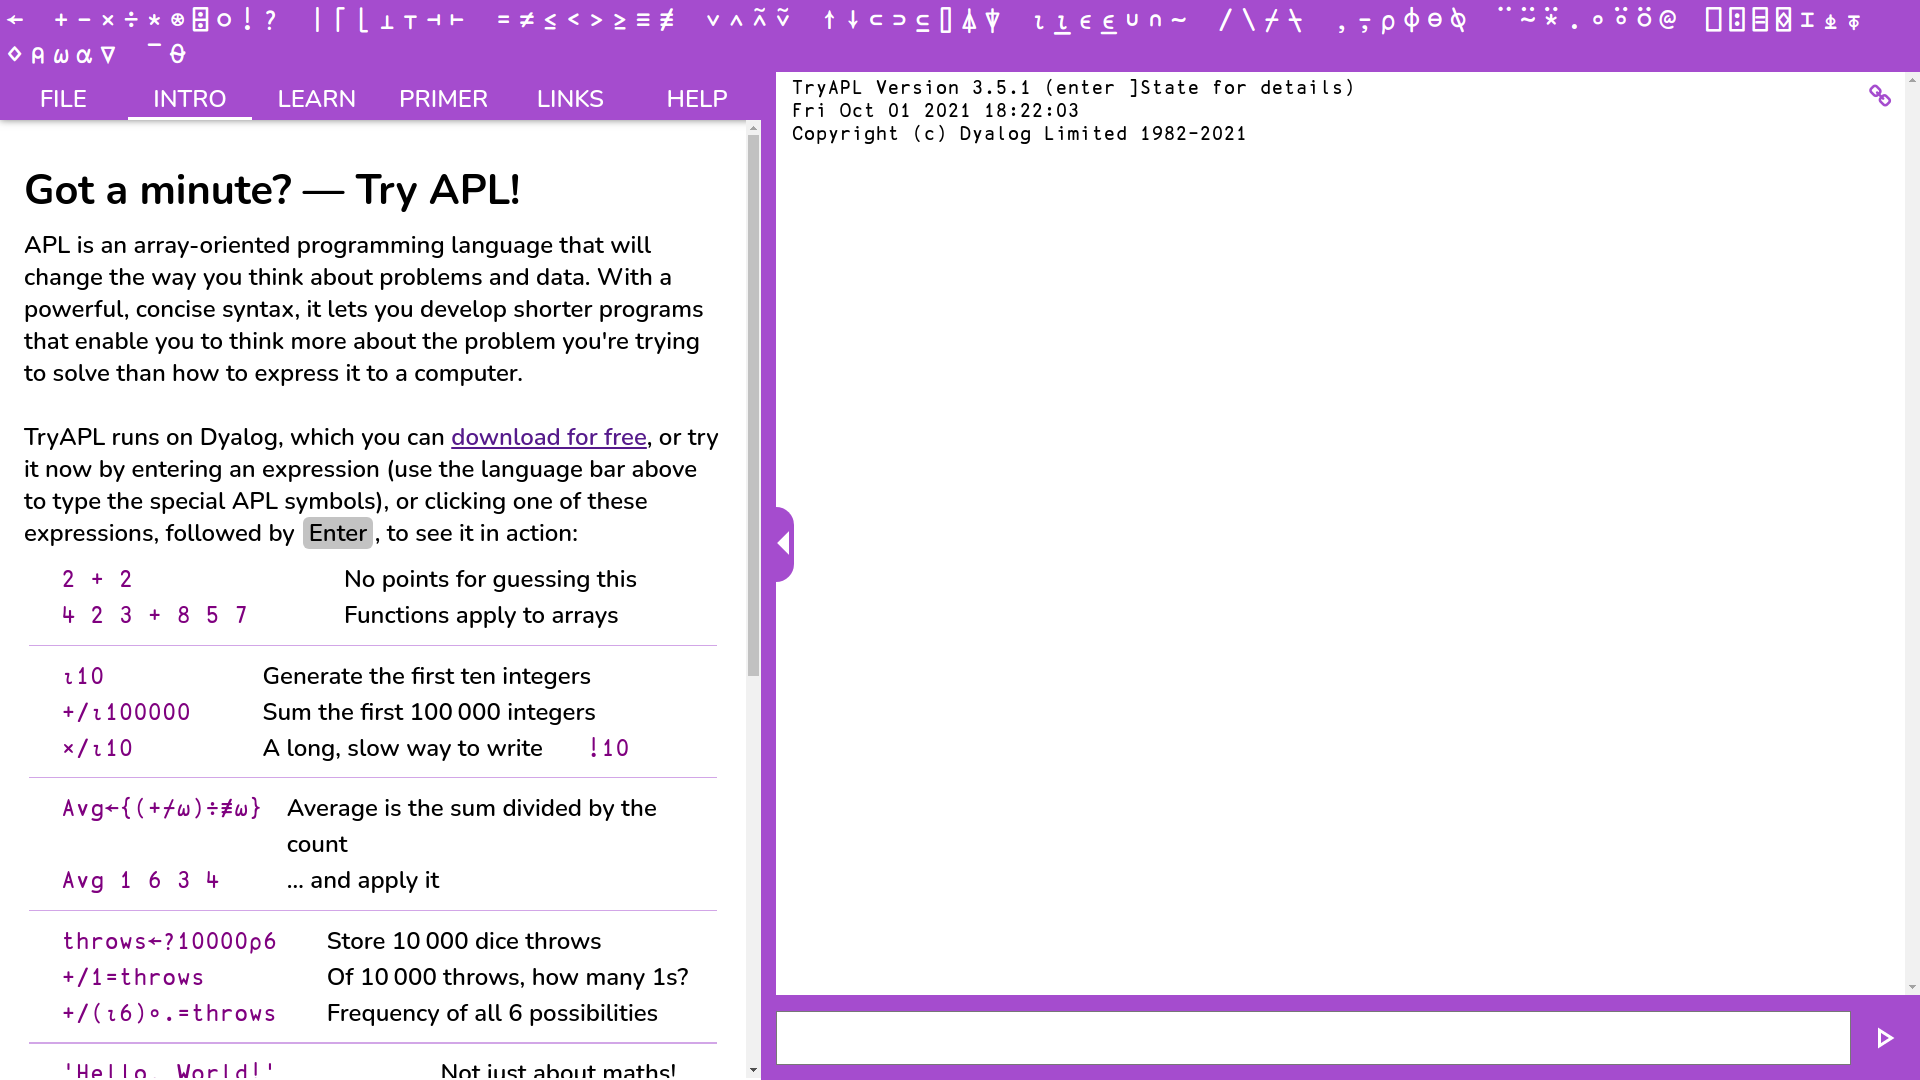
\includegraphics[scale=0.125]{figs/tryapl.png}
        \end{figure}

    \end{itemize}

\end{frame}
